% !TeX root = ../main.tex
\cleardoublepage
\chapter{引言}\label{ch:bg}



\section{课题背景}

%TODO: citation


\subsection{IC产业}

IC产业是一个国家现代工业的基础,是信息产业的核心,因此发展具有战略意义的集成电路产业以占领科技、经济和军事制高点已经成为许多国家的共识。

工信部发布的《集成电路产业“十二五”发展规划》中提出,到“十二五”末,集成电路产量超过1500亿块,销售收入达3300亿元,年均增长18\%,占世界集成电路市场份额15\%左右,满足国内近30\%的市场需求。

IC制造需要大量高技术制造装备;整个IC产业的迅速发展,也带动了IC装备制造业的发展。其中,关键制造装备的国产化是大势所趋。

IC制造工艺可分为四大类:沉积(deposition),去除(removal),布线(patterning),改性(modification of electrical properties)。常见的工艺包括PVD/CVD(物理/化学气相沉积)、等离子体刻蚀、化学机械平整化、旋转涂覆、光刻、离子移植、快速退火等。从单晶硅制成的晶圆,到最后的成品芯片,要依次经历多达300道工序。所有的IC工艺均需在严格受控的条件下进行,这需要专用设备的支持。


\subsection{静电卡盘}\label{sec:intro-echuck}

卡盘(chuck)是IC装备中的通用组件,用于夹取、搬运、或固定晶圆(wafer)及其他薄片类工件(如光刻掩模等)。依据其夹紧原理,主要可分为机械卡盘、真空吸盘和静电卡盘三种。机械卡盘需与工件保持紧固的机械接触,适用于要求不高或需要传动的场合,如搬运、旋转涂覆等;真空吸盘必须工作在大气环境下,与工件接触力极小,最适合用于搬运;静电卡盘结构、原理均复杂,但吸附力均匀稳定,且能满足各类工艺所需的额外要求,广泛用于工艺装备中。

\begin{figure}[hbt]
\centering
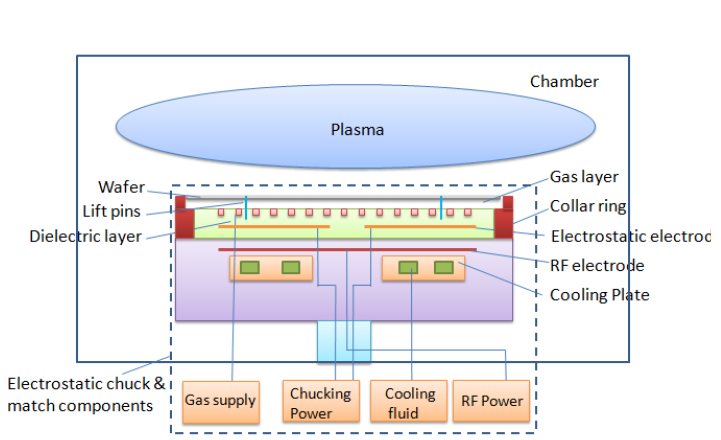
\includegraphics[width=1\linewidth]{./bg/echuck__sch.png}
\caption{静电卡盘组成示意}
\label{fig:echuck__sch}
\end{figure}

静电卡盘(如图~\ref{fig:echuck__sch})。



\section{国内外研究现状}

国内相关研究极其缺乏,在各文献数据库中均未搜索到静电卡盘静电吸引力测量的相关成果。其他静电卡盘相关的成果多为企业专利等,用于保护其独创设计。相对来说,国外对此有一定数量的研究,主要集中于静电吸附力产生机理、理论公式推导、定性实验验证、静电卡盘与工件组成系统的电学等效模型等方面。以静电力为重点的研究并不多,多数文章仅对“测量静电力”一笔带过,并未深入探究其测量手段。


\subsection{主要研究机构与企业}


\subsection{主要测量手段概述}\label{sec:priorArt}

\subsubsection{机械提拉法}\label{sec:priorArt-pull}
\subsubsection{背吹平衡法}\label{sec:priorArt-backside}
\subsubsection{变形检测法}\label{sec:priorArt-warp}



\section{论文研究内容与意义}


\subsection{工程需求}


\subsection{论文研究内容}


\subsection{对专项课题的推进作用}